\iffalse
\let\negmedspace\undefined
\let\negthickspace\undefined
\documentclass[journal,12pt,twocolumn]{IEEEtran}
\usepackage{cite}
\usepackage{amsmath,amssymb,amsfonts,amsthm}
\usepackage{algorithmic}
\usepackage{graphicx}
\usepackage{textcomp}
\usepackage{xcolor}
\usepackage{txfonts}
\usepackage{listings}
\usepackage{enumitem}
\usepackage{mathtools}
\usepackage{gensymb}
\usepackage{comment}
\usepackage[breaklinks=true]{hyperref}
\usepackage{tkz-euclide} 
\usepackage{listings}
\usepackage{gvv}                                        
\def\inputGnumericTable{}                                 
\usepackage[latin1]{inputenc}                                
\usepackage{color}                                            
\usepackage{array}                                            
\usepackage{longtable}                                       
\usepackage{calc}                                             
\usepackage{multirow}                                         
\usepackage{hhline}                                           
\usepackage{ifthen}                                           
\usepackage{lscape}

\newtheorem{theorem}{Theorem}[section]
\newtheorem{problem}{Problem}
\newtheorem{proposition}{Proposition}[section]
\newtheorem{lemma}{Lemma}[section]
\newtheorem{corollary}[theorem]{Corollary}
\newtheorem{example}{Example}[section]
\newtheorem{definition}[problem]{Definition}
\newcommand{\BEQA}{\begin{eqnarray}}
\newcommand{\EEQA}{\end{eqnarray}}
\newcommand{\define}{\stackrel{\triangle}{=}}
\theoremstyle{remark}
\newtheorem{rem}{Remark}
\begin{document}

\bibliographystyle{IEEEtran}
\vspace{3cm}

\title{GATE 2023 IN 29}
\author{EE23BTECH11065 - prem sagar}
\maketitle
\newpage

\bigskip 

\renewcommand{\thefigure}{\theenumi}
\renewcommand{\thetable}{\theenumi}
\textbf{Question}:
\\\\Let y\brak{t}=x\brak{4t},where x\brak{t} is a continous-time periodic signal of $100$s.the fundamental period of y\brak{t} is (\textbf{rounded off to the nearest integer})
 \hfill(GATE IN 29)
 \\\\\textbf{Solution}:
\fi
\begin{table}[!ht]
\def\arraystretch{1.5}
   \centering
    \renewcommand\thetable{1}
      \begin{tabular}{|c|c|c|}
   \hline
   \textbf{Symbol} & \textbf{Value}& \textbf{Description} \\
   \hline
         $T$ & $100$ & fundamental period of $x\brak{t}$\\
        \hline
        $T_1$ &  & fundamental period of y\brak{t}\\
        \hline
        $\omega_0$ & $\frac{8\pi}{100} $  & fundamental frequency of y\brak{t}\\
        \hline
\end{tabular}

    \caption{input parameters}
    \label{tab:IN 29}
 \end{table}
\\From \tabref{tab:IN 29}
\\Applying Fourier series:
 \begin{align}
 x\brak{t}&=\sum_{n=-\infty}^{\infty}c_ne^\frac{j\;2\pi n\;t}{100}
\\ y\brak{t}&=x\brak{4t}
\\ y\brak{t}&=\sum_{n=-\infty}^{\infty}c_ne^\frac{j\;2\pi n\;\brak{4t}}{100}
\\&=\sum_{n=-\infty}^{\infty}c_ne^\frac{j\;2\pi n\;t}{25}
\\T_1&=25\text{sec}
 \end{align}
\begin{figure}[h]
 \renewcommand\thefigure{1}
    \centering
    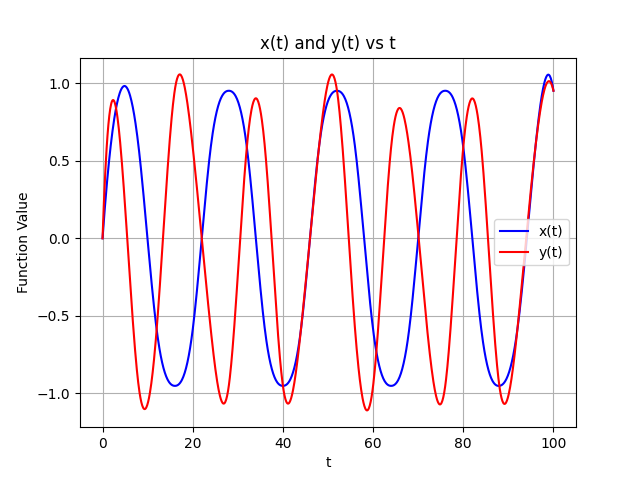
\includegraphics[width=1\linewidth]{2023/IN/29/figs/figr.png}
    \caption{plot y\brak{t} v/s t}
\end{figure}
%\end{document}
